\documentclass[journal,comsoc]{IEEEtran}

\usepackage[T1]{fontenc}% optional T1 font encoding
\usepackage[utf8]{inputenc}
\usepackage{float}
\usepackage{hyperref}
\usepackage[portuguese]{babel}
\selectlanguage{portuguese}
\usepackage{float}
\usepackage{graphicx}

\hyphenation{op-tical net-works semi-conduc-tor}


\begin{document}
	
	\title{Codificação de Canal}
	
	\author{Dylan Sugimoto, Ivan Padalko}
	
	% The paper headers
	\markboth{Relatório da disciplina ELE-32}{}
	
	% make the title area
	\maketitle
	
	\begin{abstract}
		Desenvolveu-se um programa que simula a transmissão de uma mensagem por um canal binário simétrico (\emph{Binary Symmetric Channel}, BSC). Foi estudado a influência da codificação de Hamming (nas versões 4/7 e 11/15) na redução de erros de transmissão para este canal. Propõe-se um modelo alternativo para a codificação do canal buscando a correção de erros duplos.
	\end{abstract}
	
	\section{Introdução}
		% The very first letter is a 2 line initial drop letter followed
		% by the rest of the first word in caps.
	
		\IEEEPARstart{D}{urante} a transmissão de uma mensagem por um canal não ideal, a presença de ruídos ou outras imperfeições podem alterar os sinais recebidos e, consequentemente, o conteúdo da mensagem transmitida. No caso de estarmos transmitindo uma sequência de bits, o erro da mensagem pode ser visto como a alteração de um dos bits da mensagem, ie, a recepção de um bit diferente do transmitido.
	
		Para se estudar possíveis codificações de canais, é preciso modelar de alguma forma o canal que está sendo usado e a forma em que a mensagem será transmitida. Desta forma, escolheu-se que o modelo usado seria a transmissão de uma mensagem binária (uma sequência de bits) através de um canal simétrico, ou seja, a probabilidade de um bit ser trocado é independente dos outros bits.
		
		A forma mais simples de se reduzir a probabilidade de erro é o uso de bits repetidos, ou seja, cada bit é transmitido $N$ vezes e, no momento da recepção, assume-se que o bit transmitido é o mais frequente. Porém, da mesma forma que esta codificação é simples, ela também é ineficiente sendo necessário transmitir uma mensagem $N$ vezes maior do que a mensagem de fato. 
		
		Outra forma de se reduzir o erro é o uso de bits de verificação para os bits transmitidos, ie, bits redundantes que permitem, até um certo ponto, a recuperação da mensagem transmitida em caso de um erro. Um desses métodos é o chamado código de Hamming que transmite, além dos bits que de fato compõem a mensagem, bits de paridade (ie, a aplicação de \textsc{xor} entre múltiplos bits). Um exemplo é a codificação que transmite para cada 4 bits de informação, 3 bits de paridade. Desta forma, a mensagem transmitida é dada pela multiplicação módulo 2 do vetor de bits $v$ pela matriz $G$, definida pela equação \ref{eq:HammingG}
		
		\begin{equation}
			G = \begin{bmatrix}
					1 & 0 & 0 & 0 & 1 & 1 & 1 \\
					0 & 1 & 0 & 0 & 1 & 0 & 1 \\
					0 & 0 & 1 & 0 & 1 & 1 & 0 \\
					0 & 0 & 0 & 1 & 0 & 1 & 1
				\end{bmatrix}
			\label{eq:HammingG}
		\end{equation} 
		
		Após a transmissão, pode-se multiplicar o vetor recebido pela matriz $H$, definida pela equação \ref{eq:HammingH}, e obter um vetor chamado síndrome. Caso este vetor seja nulo, assume-se que a mensagem foi transmitida corretamente. Caso contrário, este vetor indica uma quais bits podem ter sido trocados durante a transmissão e, decide-se, pelo erro de um bit que, ao ser adicionado ao vetor mensagem, geraria esta síndrome.
		
		\begin{equation}
			H = \begin{bmatrix}
					1 & 1 & 1 \\
					1 & 0 & 1 \\
					1 & 1 & 0 \\
					0 & 1 & 1 \\
					1 & 0 & 0 \\
					0 & 1 & 0 \\
					0 & 0 & 1 
				\end{bmatrix}
			\label{eq:HammingH}
		\end{equation} 
		
		De uma forma semelhante, pode-se definir as matrizes $G$ e $H$ para outros tamanhos de mensagem com quantidades diferentes de bits de verificação, por exemplo, 11 bits de mensagem para 4 bits de verificação que foi implementado nesta simulação. Este código possui taxa de $73\%$ De um modo geral, pode-se definir codificações de Hamming com $2^N-1$ bits no total com $N$ bits de verificação.
	
	\section{Descrição do algoritmo}
		
		O algoritmo implementado é composto pelas seguintes etapas:
		\begin{enumerate}
			\item Gera-se uma mensagem composta por uma sequência aleatória de bits;
			\item Codifica-se a mensagem através de algum algoritmo de codificação;
			\item Simula-se a transmissão da mensagem codificada através de um canal;
			\item Na recepção, descodifica-se a mensagem e tenta-se corrigir os erros de transmissão; 
		\end{enumerate}
	
		Na prática, utiliza-se um gerador de números aleatórios para se conseguir uma sequência de $0$s e $1$s que será considerada como a informação a ser transmitida. Após isso, a codificação de matrizes se dá pela multiplicação de uma matriz pelo vetor que compõe a mensagem. \footnote{Note que as somas que ocorrem durante a multiplicação de matrizes são módulos 2 de forma que o vetor codificado seja binário.}
		
		Para a simulação de passagem da mensagem pelo canal considera que temos um canal simétrico binário. Desta forma, considera-se que a probabilidade de ocorrer um erro de transmissão em qualquer um dos bits não depende dos demais e tem probabilidade $p$, ou seja, a probabilidade de erro de qualquer um dos bits comporta-se como uma variável de Bernoulli. Um método para simular a passagem da mensagem pelo canal se dá, portanto, pela simulação de $n$ variáveis de Bernoulli o que tem complexidade $O(n)$. Entretanto, pode-se fazer um método equivalente mais eficiente pois $n$ variáveis de Bernoulli podem ser consideradas como uma variável Binomial. Desta forma, simula-se uma variável Binomial de parâmetros $n$ e $p$ obtendo assim um valor $k$ de bits que mudariam ao se passar pelo canal e depois se escolhe ao acaso $k$ bits que terão seus valores alterados. Desta forma, temos um método de simulação de complexidade $O(1)$.
		
		Finalmente, na decodificação, multiplica-se o vetor recebido por uma matriz, calculando, assim, a síndrome. Como o erro um único bit é sempre o mais provável, associa-se a cada síndrome o erro de um bit que a geraria. Desta forma, pode-se recuperar o vetor transmitido mais provável somando o erro novamente ao vetor recebido, decodificando, portanto, a mensagem.
	
	\section{Um método para a correção de erros duplos}
		Percebe-se que há uma necessidade de se ser capaz de corrigir erros duplos (i.e. de dois bits) para se melhorar a codificação de Canal uma vez que limitou-se até então aos erros simples. Para isso, desenvolveu-se um algoritmo que que possui a mesma estrutura lógica do código de Hamming, mas adaptado para operar com 11 bits de informação e 8 bits de paridade. Portanto, esta codificação opera com taxa de $57,89\%$, ligeiramente maior  do que a taxa do código de Hamming. Desta forma, as únicas diferenças desse código com os anteriores é a forma da matriz de codificação, e, consequentemente, a forma da matriz geradora; e o algoritmo que encontra o vetor erro a	partir da síndrome.
	
		Assim, utilizou-se da estratégia de encontrar primeiro a matriz de codificação para a partir dela encontrar a matriz geradora. Para encontrar, a matriz de codificação escolheu-se para efeito de simplicidade manter a distribuição de paridade dos quatro bits que já existiam (bit 12, 13, 14 e 15), ou seja, o bit 12 continuou sendo o bit de paridade do seguinte conjunto de bits 1, 2, 3, 4, 5, 6 e 7; o bit 13, do seguinte conjunto de bits 1, 2, 3, 4, 8, 9 e 10; o bit 14, do seguinte conjunto de bits 1,2,5,6,8,9 e 11; o bit 15, do seguinte conjunto de bits 1, 3, 5, 7, 8, 10 e 11. Escolheu-se a seguinte lógica de atribuição de conjunto de bits para os outros quatro bits de paridade (bit 16, 17, 18 e 19). Para os bits de paridade que usa o bit 1, utiliza-se em seu lugar, o bit 11, para o bit 2, usou-se o bit 10, para o bit 3 usou-se o bit 9 e assim por diante gerando a tabela \ref{tab:bits}. A matriz $H$ é apresentada na equação \ref{eq:1911H}. A matriz G foi omitida devido ao seu tamanho, mas ela pode ser facilmente construída a partir da tabela \ref{tab:bits}.
		
		\begin{table*} [h]
			%% increase table row spacing, adjust to taste
			\centering
			\renewcommand{\arraystretch}{1.3}
			% if using array.sty, it might be a good idea to tweak the value of
			% \extrarowheight as needed to properly center the text within the cells
			\caption{Resultados da análise de textos escolhidos aleatoriamente}
			\label{tab:bits}
			%\centering
			%% Some packages, such as MDW tools, offer better commands for making tables
			%% than the plain LaTeX2e tabular which is used here.
			\begin{tabular}{cccccccc}
				\hline
				Bit de paridade & $1^\circ$ bit & $2^\circ$ bit & $3^\circ$ bit & $4^\circ$ bit & $5^\circ$ bit & $6^\circ$ bit & $7^\circ$ bit \\
				\hline \hline
				12 & 1  & 2  & 3 & 4 & 5 & 6  & 7 \\
				13 & 1  & 2  & 3 & 4 & 8 & 9  & 10 \\
				14 & 1  & 2  & 5 & 6 & 8 & 9  & 11 \\
				15 & 1  & 3  & 5 & 7 & 8 & 10 & 11 \\
				16 & 11 & 10 & 9 & 8 & 7 & 6  & 5 \\
				17 & 11 & 10 & 9 & 8 & 4 & 3  & 2 \\
				18 & 11 & 10 & 7 & 6 & 4 & 3  & 1 \\
				19 & 11 & 9  & 7 & 5 & 4 & 2  & 1 \\
				\hline
			\end{tabular}
		\end{table*}
	
		A ideia é que se ocorrer um erro, os conjuntos de bits de paridade da Tabela A e da Tabela B apontam para o mesmo erro de um bit. Por exemplo, se ocorrer erro no bit 1, então,	ambos os conjuntos apontam para erro no bit 1. Porém, quando ocorrer erro duplo, os quatro primeiros bits de paridade indicam erro em um determinado bit, e os outros quatro bits de paridade indicam erro em outro bit o que sinaliza que ocorreu um erro duplo na transmissão. Para encontrar, qual é o vetor erro, que tenta consertar o vetor recebido, realiza-se a soma módulo 2 da síndrome com uma linha da matriz HT, verifica-se se o resultado é uma linha da matriz de codificação, se pertencer, então o índice das duas linhas que foram somadas indicam os bits que precisam ser consertados. Se não pertencer, realiza-se a soma anteriormente citada para a próxima linha da matriz de codificação. Se após realizado a soma para todas as linhas da matriz de codificação, o resultado da soma não ter sido uma linha da matriz de codificação, então atribui-se o valor zero para o vetor de correção, ou seja, não se tenta corrigir o vetor de transmissão.
	
		É fato que essa codificação não conserta todas as combinações possíveis de erros duplos, porém os dados
		coletados mostraram que a quantidade de erros duplos que essa codificação conserta foi suficiente para obter o resultado desejado, como mostrado na seção de resultados.
		
		\begin{equation}
			H = \begin{bmatrix}
				1 & 1 & 1 & 1 & 0 & 0 & 1 & 1 \\
				1 & 1 & 1 & 0 & 0 & 1 & 0 & 1 \\
				1 & 1 & 0 & 1 & 0 & 1 & 1 & 0 \\
				1 & 1 & 0 & 0 & 0 & 1 & 1 & 1 \\
				1 & 0 & 1 & 1 & 1 & 0 & 0 & 1 \\
				1 & 0 & 1 & 0 & 1 & 0 & 1 & 0 \\
				1 & 0 & 0 & 1 & 1 & 0 & 1 & 1 \\
				0 & 1 & 1 & 1 & 1 & 1 & 0 & 0 \\
				0 & 1 & 1 & 0 & 1 & 1 & 0 & 1 \\
				0 & 1 & 0 & 1 & 1 & 1 & 1 & 0 \\
				0 & 0 & 1 & 1 & 1 & 1 & 1 & 1 \\
				1 & 0 & 0 & 0 & 0 & 0 & 0 & 0 \\
				0 & 1 & 0 & 0 & 0 & 0 & 0 & 0 \\
				0 & 0 & 1 & 0 & 0 & 0 & 0 & 0 \\
				0 & 0 & 0 & 1 & 0 & 0 & 0 & 0 \\
				0 & 0 & 0 & 0 & 1 & 0 & 0 & 0 \\
				0 & 0 & 0 & 0 & 0 & 1 & 0 & 0 \\
				0 & 0 & 0 & 0 & 0 & 0 & 1 & 0 \\
				0 & 0 & 0 & 0 & 0 & 0 & 0 & 1
			\end{bmatrix}
			\label{eq:1911H}
		\end{equation} 
		
	\section{Resultados}
		
		Gerou-se um milhão de bits aleatoriamente utilizando uma função pseudoaleatória	já implementada em \emph{Python} da biblioteca \emph{numpy} e organizou-se esses bits em vetores de 4 bits, que foram passados na função que simula o canal BSC. Assim, a quantidade de bits alterados após a passagem pelo canal é a quantidade de erro causados pelo canal e a probabilidade de	erro sem codificação é essa quantidade de erro divido por um milhão, que se apresenta na cor amarela na Figura \ref{fig:A}. O mesmo foi feito com a codificação de Hamming, a menos da	diferença que na codificação de Hamming, codificou-se o	vetor de quatro bits com a codificação Hamming, ou seja, os vetores transmitidos são de 7 bits em que 4 bits são de informação e 3 bits são de verificação de paridade. E após a passagem pelo canal BSC, decodificou-se e os erros presentes nos bits de informação foram contabilizados. Igualmente para o caso sem codificação fez esse processo para vários valores de probabilidade de erro de um bit, começando com probabilidade de $50\%$ de erro de um bit após passagem pelo canal BSC até a perda da capacidade de medição, que é quando a probabilidade de erro vai a zero, ou seja, a decodificação consegue consertar todos os erros que aparecem	após passagem pelo canal BSC, e assim, não se contabiliza nenhum erro. Esse momento da perda da capacidade de medida está marcado na Figura \ref{fig:A} com uma reta quase vertical.
		
		\begin{figure}[hbt]
			\centering
			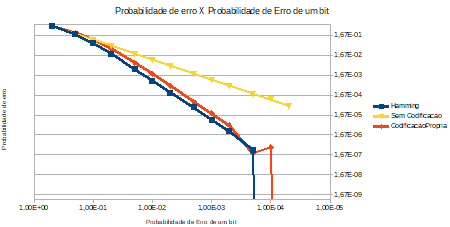
\includegraphics[width=\columnwidth]{../img/PeXp.png}%
			\caption{Gráfico log-log da probabilidade de erro de transmissão pela probabilidade de erro de bit}%
			\label{fig:A}%
		\end{figure}
		
		A mesma situação de repete para a codificação adaptada do código de Hamming para transmissão de 11 bits de informação e 4 bits de paridade, ou seja, gerou-se 999.999 bits	aleatoriamente, e organizou-se em vetores de 11 bits. Porém, observa-se que a probabilidade de erro da codificação adaptada (curva vermelha da Figura \ref{fig:A}), é maior para quase todos os valores de probabilidade de erro de um bit, a exceção	de um ponto que ocorre para probabilidade de erro de um bit	igual à $2\cdot 10^{-4}$, que pode ser desconsiderado devido à alta variância da medida para esse caso, o que significa que depende da medida, esse ponto pode ficar tanto acima quanto a baixo da curva azul, pois quantidade de erros que ocorre é muito pequena. O principal é compreender que a curva da codificação adaptada de Hamming fica acima da curva do código de Hamming porque o vetor transmitido no caso da codificação adaptada é de tamanho 15 enquanto que no código de Hamming, o tamanho do vetor transmitido é 7 o que implica pelo fato da quantidade de erros que ocorre após	passagem pelo canal BSC ser uma distribuição binomial que o vetor transmitido de tamanho maior tem probabilidade de erro múltiplo, que é quando ocorre mais de um erro no vetor	transmitido, maior do que o vetor menor, como se observa na	Figura \ref{fig:C}. Assim, como o código adaptado conserta apenas um erro, da mesma forma que o código de Hamming só conserta um erro, tem-se que a probabilidade de erro da codificação adaptada (curva vermelha) é maior que a probabilidade de erro da codificação de Hamming, apesar de ter se observado mais erros ocorrerem após passagem pelo canal e antes da decodificação para o código de Hamming do que para o código adaptado, como se observa na Figura \ref{fig:B}. Assim, em termos de probabilidade de erro, a codificação de Hamming é melhor do que a adaptada.
		
		\begin{figure}[hbt]
			\centering
			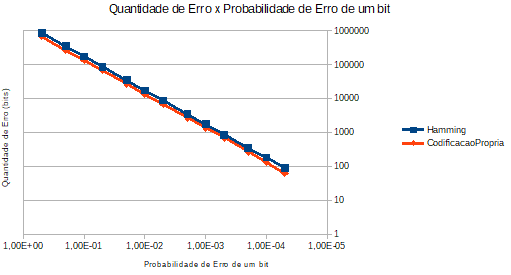
\includegraphics[width=\columnwidth]{../img/QuantErroXp.png}%
			\caption{Quantidade de erros total após passagem pelo canal BSC e antes da decodificação por probabilidade de erro de um bit}%
			\label{fig:B}%
		\end{figure}
				
		Dessa forma, percebeu-se que para se ter uma melhor performance do que o código de Hamming em termos de probabilidade de erro, é necessário que a codificação utilizada	consiga detectar e corrigir dois erros na etapa de decodificação, se o vetor transmitido tiver tamanho maior do que o código de Hamming, que é o desejado neste estudo. Assim, adicionou-se mais quatro bits de paridade para tentar	realizar a detecção e correção de erros duplos, que ocorre quando há dois erros no vetor transmitido, chegando-se assim ao código 1911 (em verde na Figura \ref{fig:D}), que não corrige todos os erros duplos possíveis, mas o subconjunto dos erros duplos que esse código corrige é suficiente para ter uma performance melhor do que o código adaptado, praticamente, para todo valor de probabilidade de erro de um bit, e do que o código de Hamming, a partir de $5 \cdot 10^{4}$, como se observa na Figura \ref{fig:D}.
		
		\begin{figure}[hbt]
			\centering
			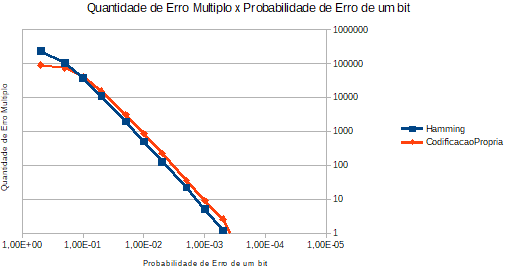
\includegraphics[width=\columnwidth]{../img/QuantErroMultXp.png}%
			\caption{Quantidade de erro múltiplo após passagem pelo	canal BSC e antes da decodificação por probabilidade de erro de um bit.}%
			\label{fig:C}%
		\end{figure}
	
		\begin{figure}[hbt]
			\centering
			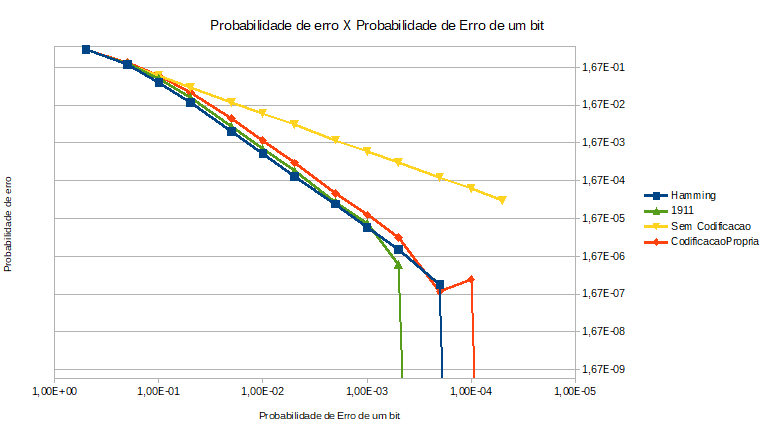
\includegraphics[width=\columnwidth]{../img/PeXp_1911.png}%
			\caption{Gráfico log-log da probabilidade de erro de transmissão pela probabilidade de erro de bit incluindo a codificação 1911}%
			\label{fig:D}%
		\end{figure}]
		
		Na Figura \ref{fig:D}, tem-se a relação entre o tamanho do bloco e o desempenho, ou seja, dividiu-se os valores de probabilidade de erro encontrados e dividiu-se pelo tamanho do vetor transmitido. Nesse caso, a curva da codificação 1911 ficou menor que as demais, pois o seu vetor transmitido é maior (19 bits), e a sua probabilidade de erro não é tão maior do que as	3 demais codificações proporcionalmente ao tamanho do vetor. No caso da codificação adaptada de Hamming para transmissão de 15 bits, inicialmente o valor é menor do que o Hamming 4/7 porque o seu vetor é maior e as probabilidades	de erros são bem próximas (vide Figura \ref{fig:A}). Depois, essas duas curvas se aproximam, pois a probabilidade de erro da codificação Hamming diminui mais do que a codificação adaptada. Assim, observou-se que quanto maior o tamanho do vetor maior é a probabilidade de erro, ou seja, menor é o desempenho para códigos que corrigem apenas um bit de erro, e supondo o canal seja BSC. Isso ocorre porque a probabilidade de erro múltiplo aumenta com o aumento do tamanho do vetor, como se observa na Figura \ref{fig:F}. Assim, é necessário aumentar a quantidade de erros corrigíveis ao aumentar o tamanho do vetor para se ter um desempenho melhor, como ocorreu no código 1911 em que se corrigiu um subconjunto dos erros duplos além dos erros simples, quando ocorre apenas um erro.
		
		\begin{figure}[hbt]
			\centering
			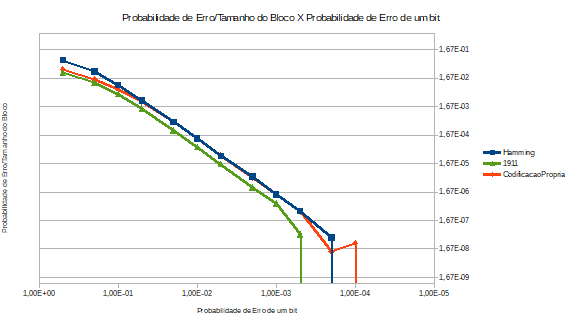
\includegraphics[width=\columnwidth]{../img/Tamanho_Desempenho.png}%
			\caption{Probabilidade de erro de cada codificação divido pelo tamanho do vetor codificado transmitido por valor de probabilidade de erro de um bit para o canal BSC}%
			\label{fig:E}%
		\end{figure}
	
		\begin{figure}[hbt]
			\centering
			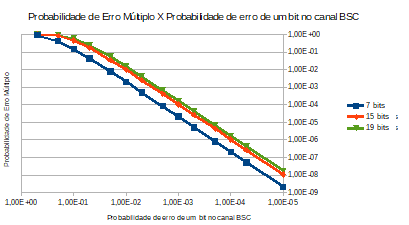
\includegraphics[width=\columnwidth]{../img/binominal_erro_multiplo.png}%
			\caption{Probabilidade de erro múltiplo para diferentes tamanhos de vetores transmitidos por probabilidade de erro de um bit ao passar pelo canal BSC}%
			\label{fig:F}%
		\end{figure}
			
		Na Figura \ref{fig:G}, percebe-se que as três primeiras medidas de	probabilidade de erro realizadas foram feitas com taxa maior do que a capacidade do canal o que significa que não existe uma codificação que consiga diminuir a probabilidade de erro para um valor tão baixo quanto se queira, mas depois da terceira medida, a taxa fica menor do que a capacidade do canal o que significa que existe uma codificação que diminua	a probabilidade para tão baixo quanto se queira.
		
		\begin{figure}[hbt]
			\centering
			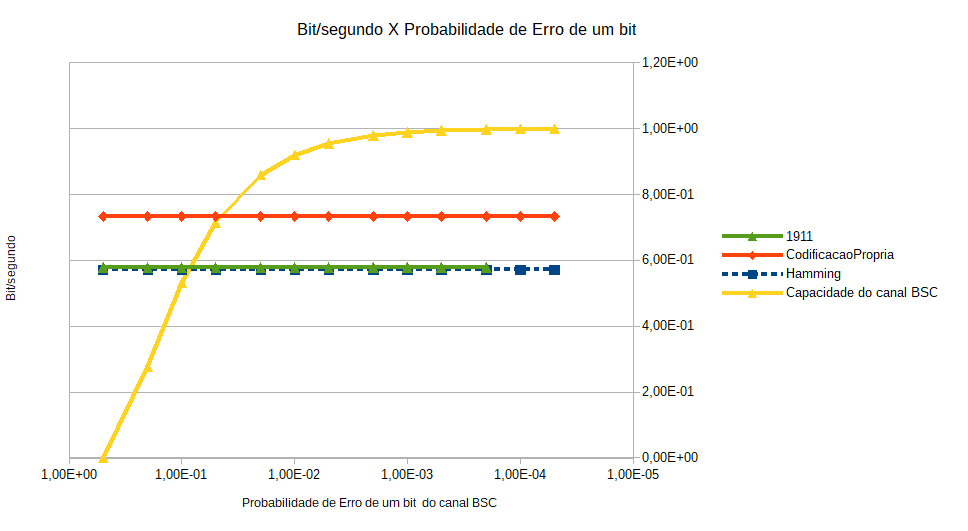
\includegraphics[width=\columnwidth]{../img/Capacidade_Canal.png}%
			\caption{Quantidade de bits de informação por tamanho do vetor transmitido (taxa), e capacidade do canal BSC. O eixo das abscissas está em escala logarítmica}%
			\label{fig:G}%
		\end{figure}
	
	\section{Conclusão}
		
		Conclui-se com este estudo que a codificação de Hamming 74 é bastante eficiente mesmo que seja bastante simples. Pode-se ver que apenas aumentar a quantidade de bits pode ser pior pois isto acarreta uma probabilidade maior de ocorrer erros duplos. A codificação desenvolvida propõe um método simples de lidar com esse caso apresentando uma taxa próxima da codificação de Hamming mas com uma probabilidade de erro menor especialmente quando a probabilidade de erro é baixa.
	
	\appendices
	
	\section{Erro por razão sinal ruído}
	\begin{figure}[H]
		\centering
		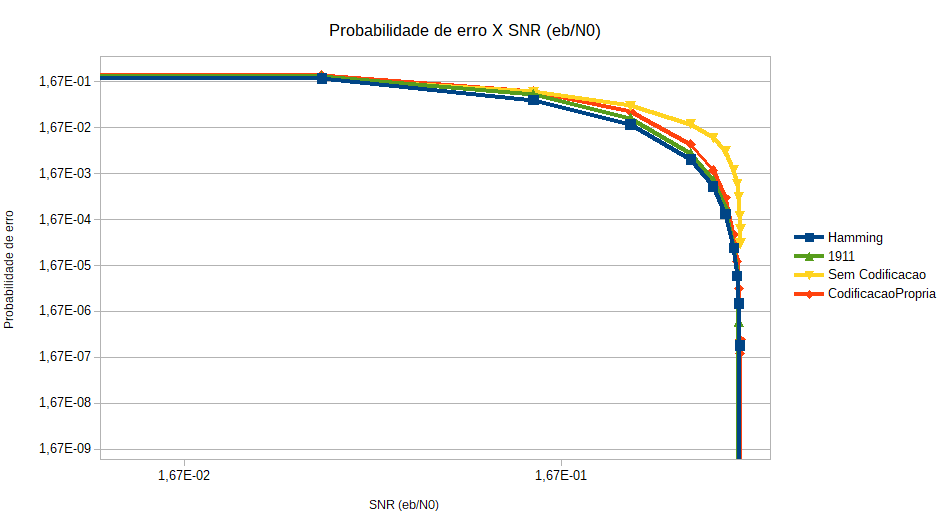
\includegraphics[width=\columnwidth]{../img/SNR_Pe.png}%
		\caption{Gráfico log-log da probabilidade de erro por razão sinal ruído}%
		\label{fig:A1}%
	\end{figure}
	
	\section{Código fonte do programa}
	O código fonte e os textos utilizados estão disponíveis \href{https://github.com/DylanNS/LAB-3_ELE-32_2017}{neste repositório do github.}
	
\end{document}


